\documentclass[border=6pt]{standalone}
\usepackage{tikz}
\usetikzlibrary{arrows.meta,positioning,calc,shapes.geometric,fit,backgrounds,patterns,matrix,decorations.pathreplacing}
\begin{document}
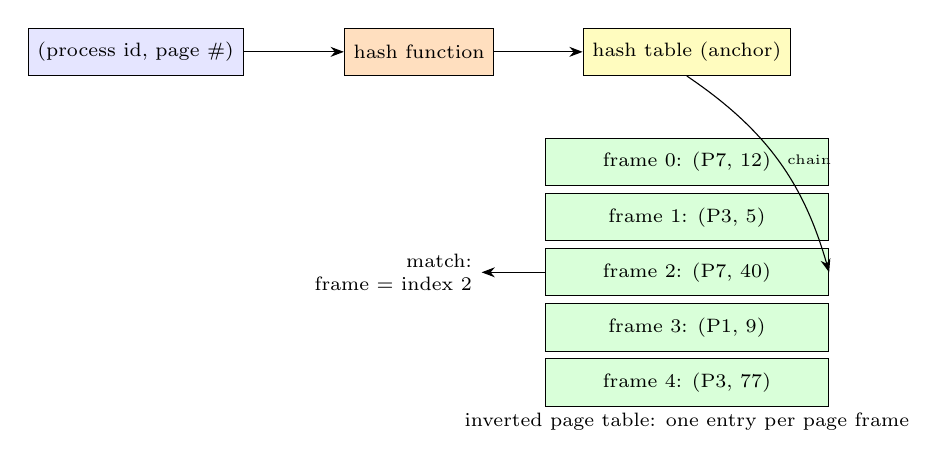
\begin{tikzpicture}[>=Stealth,font=\small]
\tikzstyle{b}=[draw,minimum height=0.6cm,font=\scriptsize]
\node[b,fill=blue!10,minimum width=2.6cm] (v) at (0,2) {(process id, page \#)};
\node[b,fill=orange!25,minimum width=1.8cm] (h) at (3.6,2) {hash function};
\node[b,fill=yellow!25,minimum width=2.6cm] (ht) at (7,2) {hash table (anchor)};
\draw[->] (v) -- (h); \draw[->] (h) -- (ht);
\foreach \i/\t in {0/{frame 0: (P7, 12)},1/{frame 1: (P3, 5)},2/{frame 2: (P7, 40)},3/{frame 3: (P1, 9)},4/{frame 4: (P3, 77)}} \node[b,minimum width=3.6cm,fill=green!15] (f\i) at (7,0.6-\i*0.7) {\t};
\node[font=\scriptsize] at (7,-2.7) {inverted page table: one entry per page frame};
\draw[->] (ht.south) to[bend left=20] node[right,font=\tiny]{chain} (f2.east);
\draw[->] (f2.west) ++(0,0) -- ++(-0.8,0) node[left,font=\scriptsize,align=right]{match:\\ frame = index 2};
\end{tikzpicture}
\end{document}
